\documentclass[12pt]{amsart}

\usepackage{amsmath}
\usepackage{amsfonts}
\usepackage{amssymb}
\usepackage[utf8]{inputenc}
\usepackage{listings}
\usepackage[pdftex]{hyperref}
\usepackage{caption}
\usepackage{subcaption}
\usepackage{geometry}
\geometry{
 letterpaper,
 total={8.5in,11in},
left=25mm,
right=25mm, 
top=20mm,
bottom=20mm,
}
 \usepackage{setspace}
\doublespace 
\usepackage[document]{ragged2e}

\usepackage{helvet}
\renewcommand{\familydefault}{\sfdefault}

\usepackage{blindtext}

\usepackage[spanish]{babel}

\usepackage{graphicx}
\usepackage{epsfig}

\begin{document}

\begin{center}
    {\large Proyecto Final de Inteligencia Artificial y Simulación}  \\ 
	 \vspace{0.5cm}  
    \vskip 0.1cm
    {\LARGE \textbf{World of Needs}} \\
    \vskip 2cm
    {\Large Autores (Grupo C-311):}\\ 
    \vspace{0.5cm} 
    		{\Large\textbf{David Manuel García Aguilera}} \\
    		{\normalsize\textit{Usuario en Github: @dmga44}}\\
 			{\Large\textbf{Rolando Sánchez Ramos}}\\
 			{\normalsize\textit{Usuario en Github: @rolysr}}\\
			{\Large\textbf{Andry Rosquet Rodríguez}}\\
 			{\normalsize\textit{Usuario en Github: @aXoXoR2}}\\
	 \vspace{1cm}
	{\Large Repositorio en Github:}\\
	{\url{https://github.com/rolysr/world-of-needs}}\\  
 	\vspace{0.5cm}
	{\large Curso 2022}  \\ 
	 \vspace{0.5cm}   
  \vskip 20cm
  
  \Large \textbf{Resumen}:
    En las sociedades humanas actuales se manifiestan diariamente procesos de movimientos de personas con diversos objetivos. Un ejemplo bastante importante es el que realizan algunos actores sociales con el fin de buscar víveres y realizar trámites de manera general para satisfacer una serie de necesidades personales o de su hogar. Las instituciones encargadas de velar por la satisfacción de los pedidos básicos de los habitantes de una zona determinada, invierten en recursos y medios correspondientes a estos pedidos, además de planificar la forma de acceso a los mismos por parte de los pobladores. El objetivo de este proyecto es permitir simular un sistema que defina el comportamiento de una sociedad o conjunto de personas distribuidas a lo largo de una zona acotada, donde existen una serie de centros especiales a los que estos humanos deben trasladarse para satisfacer sus necesidades, con lo cual se permitirá dar respuesta a problemáticas relacionadas con la cantidad de dinero a invertir por una entidad central a cargo de los centros de destino y el grado de satisfacción de un conjunto de clientes potenciales.

  \end{center}
  


\newpage
\section{Introducci\'on}
El problema que se abordará en este proyecto tiene inicialmente una entidad central (organización gubernamental, empresa o institución), la cual posee un conjunto de destinos (centros comerciales, tiendas, institutos) en los que se puede dar solución a una o más necesidades predefinidas (venta de alimentos, víveres del hogar y otros productos, tramitación de documentos). Se tiene además, un espacio acotado donde estarán localizados cada uno de los centros adjuntos de dicha entidad, el cual puede ser considerado como una porción de una ciudad. También, es conocido el presupuesto con que la misma cuenta para adquirir los productos o soluciones que puede brindar a manera de ofertas, de forma tal que estas puedan ser distribuídas de alguna forma en los destinos posibles. En el problema se tiene en cuenta la presencia de una serie de clientes, los cuales son personas que poseen necesidades que pueden ser ofertadas en algunos de los centros establecidos. Por lo tanto, uno de los objetivos principales de este trabajo consiste en simular el proceso mediante el cual un conjunto de personas se traslada en una región con presencia de destinos posibles, con el fin de satisfacer sus necesidades, para lo cual se propone un modelo basado en múltiples agentes.

	El modelado basado en agentes es una metodología computacional que nos permite crear, analizar y experimentar con mundos artificiales poblados por agentes con disímiles comportamientos y objetivos. Existen varias áreas de investigación relacionadas con el modelado basado en agentes para la simulación del efecto de los cambios en el entorno a partir del movimiento de las personas \cite{soa1} \cite{soa2}, las cuales pueden contar con una serie de necesidades y/o formas de actuar, como por ejemplo en modelos a microescala \cite{soa3} \cite{soa4}, los cuales constituyen una interesante solución para agentes que poseen una planificación bien definida de la forma en que deciden satisfacer sus necesidades. Otros estudios referentes al comportamiento de agentes que se trasladan para realizar compras a nivel regional \cite{soa5} resultan interesantes pues se introducen conceptos como índices de calidad de un destino en base a las necesidades, la distancia y la calidad de las ofertas, así como características propias de los agentes, como la edad, el índice de ingresos monetarios y la distribución de sus necesidades.

Finalmente, teniendo en cuenta las investigaciones en el campo de simulaciones de multiples agentes en ciudades con una planificación de compras en base a necesidades, se propone establecer un modelo computacional que permita, a partir de un conjunto de centros de destino, agentes con necesidades predefinidas, verificar interrogantes como: ¿De qué forma se pudiera distribuir un presupuesto inicial para construir lugares de destinos en un ambiente dado con el fin de satisfacer la mayor cantidad de necesidades de los agentes en este? ¿Cuánto presupuesto haría falta para satisfacer la necesidad de todos? ¿Cuál es el mínimo presupuesto para satisfacer a una cantidad especificada de ciudadanos con cierto margen de error? Por lo tanto, podemos ver inicialmente la utilidad de esta propuesta.

\section{Desarrollo}

Al analizar los requerimientos del problema planteado, vemos una serie de componentes principales que resulta evidente implementar, así como un conjunto de funcionalidades que estas deberían ofrecer y las relaciones que se manifiestan entre las mismas. Por lo tanto dichas componentes serían:

•	Ambiente: Representa el medio sobre el cual se llevarán a cabo los sucesos de la simulación. El mismo deberá tener una forma de almacenar o representar el estado geográfico de los componentes que este contiene y de los hechos que en él ocurren. Una forma de representación de este pudiese ser a partir de una matriz bidimensional con celdas que representen una unidad de espacio que puede ser válida o no para la presencia y recorrido de los agentes o la creación de centros posibles de destino para estos.

El ambiente debe tener funcionalidades como:
\begin {enumerate}
			\item Añadir agentes y centros en posiciones válidas y almacenar datos referentes a estos de alguna forma.
			\item Ofrecer datos suficientes del estado geográfico para ser utilizados por un framework dedicado a la visualización de mapas o zonas.
			\item Calcular y llevar internamente estadísticas que permitan describir el estado de los componentes y hechos en el sistema como por ejemplo el tiempo transcurrido.
\end {enumerate}

•	Lugares de destino: Estos componentes pueden representar desde una tienda de productos hasta un centro para que los agentes realicen algún trámite. Los mismo deben estar ubicados en zonas específicas del mapa y ofrecer una descripción de las necesidades que pueden ser satisfechas ahí. 

Para cada necesidad posible en un lugar de destino habrá una forma específica de tratar a los agentes que arriban. Un ejemplo de esto puede ser un lugar de destino $D1$, al cual se le define una necesidad $N1$ con ciertas características como límite de disponibilidad, el cual atiende a los clientes con una política de colas bien definida.

Las posibles funcionalidades de los lugares de destino son:
\begin {enumerate}
			\item Llevar un estado interno del sistema siendo simulado y que contenga estadísticas que permitan analizar el estado actual.
			\item Definir una política mediante la cual serán atendidos los clientes, por ejemplo, la cantidad de servidores de atención, si estos servidores son en serie o paralelo.
			\item Definir una forma mínima de almacenamiento del estado de los clientes inmersos en el proceso de espera.
\end {enumerate}

•	Agentes: Son aquellos integrantes del sistema que tienen como objetivo simular el comportamiento humano y tomar decisiones en base a una serie de objetivos predefinidos en los mismo. Estos pueden tener una serie de límites como dinero disponible, cantidad de necesidades a cumplir. 

Las funcionalidades que pueden tener estos son:
\begin {enumerate}
			\item Definir límites de los mismo en cuanto a diversos parámetros como capacidad monetaria y necesidades.
			\item Definir política o forma de comportamiento, lo cual influye en el proceso de toma de decisiones como decidir a dónde moverse etc.
			\item Tener formas de mostrar el estado de su satisfacción en base a los objetivos cumplido y que se pueda conocer los que le faltan por cumplir.
\end {enumerate}

\subsection{Implementación del modelo propuesto:} 

\paragraph{Para llevar a cabo la simulación se implementaron un conjunto de módulos principales, utilizando el lenguaje de programación \textit{Python} \cite{python}. Dichos módulos son: \textit{agents} , \textit{environments} y \textit{utils}, los cuales contienen aquellos tipos de datos y funciones necesarias para ejecutar todos los procesos pensados para este proyecto. El módulo \textit{agents} está destinado para la implementación de los tipos de agentes que intervienen en la simulación, así como el conjunto de campos, propiedades y métodos necesarios para su correcto funcionamiento en un entorno. Por otro lado, el módulo \textit{environments} tiene como objetivo crear tipos de datos que permitan representar un entorno de ejecución, colocar agentes, verificar el estado de la simulación, llevar a cabo un conjunto de iteraciones, entre otras funcionalidades. Finalmente, se tiene el módulo \textit{utils}, que contiene a su vez submódulos encargados de la generación de grafos en forma de ciudades, generación de variables aleatorias que representen algunos hiperparámetros de la simulación (como por ejemplo la velocidad de desplazamiento de las personas en una ciudad), algoritmos de decisión de los agentes para determinar la próxima acción a realizar y las políticas de comportamiento de los agentes para realizar las compras o adquisición de medios en un lugar de destino.}

\paragraph{Los módulos \textit{agents} y \textit{environments} dependen de implementaciones en \textit{utils}, mientras que en un segundo plano, pero no menos importante, se tiene el módulo \textit{testing}, el cual está orientado a la implementación de pruebas unitarias e integración entre los tres módulos principales. En la figura \ref{fig:architecture} se muestra la arquitectura general de los módulos del proyecto y la dependencia entre estos:}

\begin{center}
	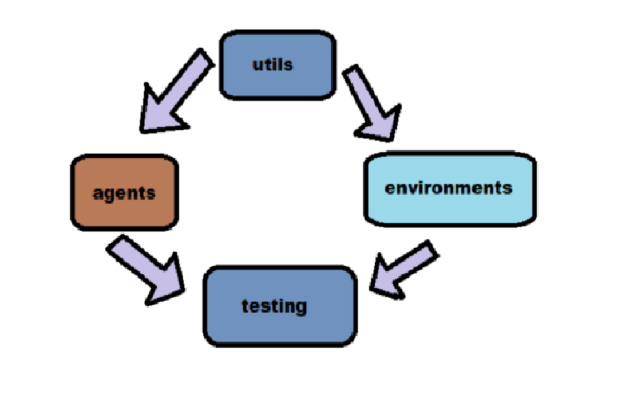
\includegraphics[scale=0.8]{./images/architecture.png}
	\captionof{figure}{Arquitectura del proyecto.}\label{fig:architecture}
\end{center}
\vskip 1.5cm

	\subsubsection{Módulo \textit{agents}:}\label{subsubsec:agents}

	\paragraph{El módulo \textit{agents} contiene las especificaciones de los tipos de agentes que intervendrán durante la simulación. Inicialmente se tiene la implementación de la clase \textit{Agent}, que representa la clase base que contiene todas las funcionalidades comunes mínimas de cualquier tipo de agente que se desee implementar para el proyecto, esta posee los campos: \textit{id} (identificador único del agente en el entorno), \textit{log\_record} (lista de descripciones de las acciones del agente durante su ejecución), \textit{name} (forma legible de identificar a un agente). Además, esta clase tiene el método \textit{narrate}, el cual es utilizado para imprimir las acciones de un agente en un determinado intervalo de tiempo desde que este comenzó a ejecutarse en una simulación.}

\paragraph{La clase \textit{HumanAgent} hereda de \textit{Agent}, y la misma representa a los agentes humanos. Los campos principales que contiene son: \textit{needs} (contiene una lista de las necesidades del agente, las cuales contienen la prioridad, un identificador y la cantidad a satisfacer), \textit{speed} (velocidad de traslación del agente en el entorno en metros por minuto), \textit{balance} (capacidad monetaria del agente humano), \textit{social\_class} (clase social del agente humano, determina su política de compra). También, esta clase contiene el método \textit{offers\_requests}, el cual recibe un conjunto de ofertas de varias posibles necesidades y en base a su clase social, ejecuta una lógica que consiste en seleccionar un conjunto de ofertas de tal forma que satisfaga sus necesidades en base a un criterio particular. Otro de los métodos importantes es \textit{next\_destination\_to\_move}, con el cual el agente humano decide, dado su estado actual y su percepción del entorno, cuál sería el próximo destino al cual dirigirse para satisfacer sus requerimientos personales. Los agentes humanos poseen también una forma de determinar la calidad de las compras que realizar así como el grado de satisfacción dado el estado actual, lo cual es determinado por los métodos \textit{purchase\_dissatisfaction} y \textit{dissatisfaction} respectivamente. En un segundo plano se encuentra el método \textit{reset}, que es utilizado para reestablecer los valores del agente humano exactamente como los tenía al inicio de su creación.}

\paragraph{El tipo definido \textit{DestinationAgent} permite representar a los destinos posibles a los que pueden acudir los agentes humanos. Los campos principales de estos son: \textit{offers} (conjunto de ofertas del destino, las cuales contienen un identificador de la necesidad que satisface, la cantidad que ofrecen y el precio al cual ofrecen cada unidad), \textit{total\_time\_working} (tiempo en que está disponible un destino, dado en horas) y \textit{queue} (forma interna de dar seguimiento al estado interno de los clientes y determinar quién es el próximo a ser atendido). Para determinar tiempo de atención a un cliente se utiliza el método \textit{attention\_time} el cual devuelve el resultado de alguna variable aleatoria que represente este fenómeno en minutos. También, esta clase contiene el método \textit{process\_offers\_requests}, el cual recibe un conjunto de solicitudes de ofertas de un agente humano y se encarga de internamente actualizar el estado del destino. Análogamente a \textit{HumanAgent}, esta clase posee el método \textit{reset} cuya implementación sigue el mismo principio que en dicho caso.}

\paragraph{En la figura \ref{fig:agentsmod} vemos un ejemplo de la manera en que se expresan las dependencias y principales características de las clases en este módulo.}

\begin{center}
	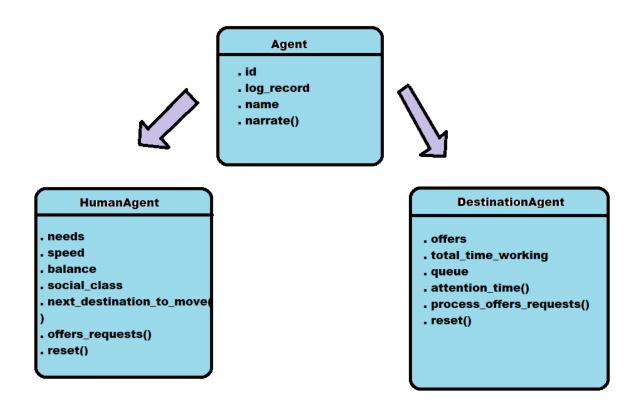
\includegraphics[scale=0.8]{./images/agentsmod.png}
	\captionof{figure}{Módulo \textit{agents}.}\label{fig:agentsmod}
\end{center}

\subsubsection{Módulo \textit{environments}:}

\paragraph{Con el módulo \textit{environments} se logra representar los posibles entornos donde podrían intervenir los agentes implementados y realizar ejecuciones de los mismos para obtener resultados que permitan arribar a conclusiones de una simulación particular. Para ello, se cuenta con las implementaciones de las clases \textit{Environment} y \textit{Experiment}}

\paragraph{La clase \textit{Environment} es una implementación genérica de los posibles entornos que pueden ser probados para la ejecución. Sus campos principales son: \textit{human\_agents} (conjunto de instancias de los agentes humanos), \textit{destination\_agents} (conjunto de instancias de los agentes de destino), \textit{graph} (grafo interno del entorno que representa una ciudad) y \textit{schedule} (cola de prioridad interna con el conjunto de acciones que deben ocurrir en la simulación). También, unido a dichos campos se encuentran métodos como \textit{execute} y \textit{run}, donde el primero recibe un parámetro que representa el tiempo en minutos a simular dado el estado actual del entorno y ejecuta los procesos que pueden ocurrir en dicho intervalo de tiempo, mientras que el segundo se encarga de correr toda la simulación mientras queden acciones por realizarse o el tiempo de ejecución del sistema no haya terminado. Para determinar que el sistema ya completó todo el proceso de simulación se implementó el método \textit{is\_done}, que básicamente comprueba que el tiempo de ejecución predefinido para el entorno no se haya cumplido. Además, resulta importante destacar los métodos \textit{negotiation} y \textit{arrival}, los cuales son utilizados para ejecutar los dos tipos de acciones fundamentales que pueden ocurrir en el entorno, la negociación de un humano con un centro de destino y la llegada de un agente a un centro de destino. Por otro lado, al igual que en las clases del módulo \textit{agents}, se tienen implementaciones para los métodos \textit{narrate} y \textit{reset}.}

\paragraph{Por último, se tiene la implementación del tipo \textit{Experiment}, cuya función es ejecutar repetidamente un entorno predefinido, de tal forma que en cada iteración se varíen algunos hiperparámetros escogidos de este con el fin de dar respuestas a las posibles interrogantes que se esperan solucionar con este proyecto. Básicamente esta clase recibe una instancia del tipo \textit{Environment} y con los métodos de optimización que tiene implementado, permite definir si se quiere optimizar los parámetros del entorno en base a un factor predefinido. Estos factores de optimización están especificados en un \textit{enum} denominado \textit{optimization\_target}, el cual contiene los factores:} \label{par:exp}
\begin {enumerate}
				\item {STORE\_OFFERS\_DENSITY: Optimización de la densidad de las ofertas en los lugares de destino.}
				\item {OFFERS\_PRICE\_FACTOR: Optimización de los precios de los productos en los destinos.}
				\item {TOTAL\_BUDGET\_FACTOR: Optimización del presupuesto de la entidad central a cargo de los destinos.}
				\item {STORE\_DISTRIBUTION: Optimización de la proporción del suministro de los destinos en el entorno.}
\end {enumerate}

\paragraph{La ejecución del proyecto se basa principalmente en la clase \textit{Experiment}, la cual depende de una implementación específica del tipo \textit{Environment}. Aunque los entornos puedan ser ejecutados de forma independiente, es mediante los experimentos que se logra encontrar sentido a los posibles resultados que puedan derivarse de la simulación. Un ejemplo de la arquitectura de este módulo se muestra en la figura \ref{fig:envsmod}}

\begin{center}
	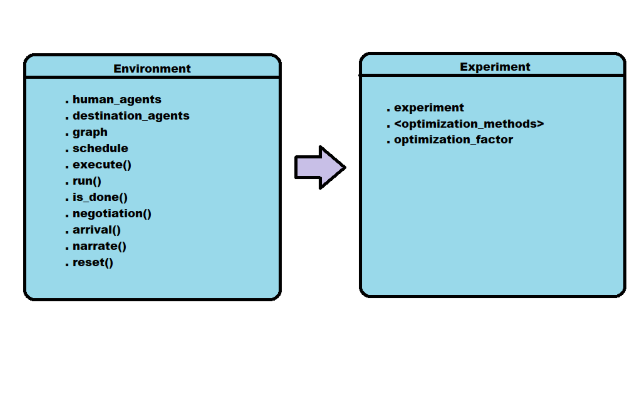
\includegraphics[scale=0.8]{./images/envsmod.png}
	\captionof{figure}{Módulo \textit{environments}.}\label{fig:envsmod}
\end{center}

\subsubsection{Módulo \textit{utils}:}

\paragraph{En este módulo se encuentran varios submódulos encargados de muchas de las funcionalidades añadidas a los módulos \textit{agents} y \textit{environments}: }

		\begin{enumerate}
			\item \textit{generator}: Contiene todos las implementaciones de los hiperparámetros, estructuras de datos y variables aleatorias generadas para la simulación.
			\begin {enumerate}
				\item {\textit{destination\_generators}: Generadores de los agentes de destino.}
				\item {\textit{human\_generators}: Generadores de los agentes humanos.}
				\item {\textit{natural\_language\_generation}: Generación de los nombres de los agentes humanos y de destino.}
				\item {\textit{environment\_schedule\_generator}: Generación del orden de las acciones iniciales en un entorno.}
				\item {\textit{graph\_generator}: Generación de los grafos de las ciudades donde se ejecutarán las simulaciones.}
				\item {\textit{street\_length\_generator}: Generación del tamaño de las calles de las ciudades.}
			\end {enumerate}
			\item \textit{graph}: Implementaciones para representar el estado de los grafos de las ciudades
			\begin {enumerate}
				\item {\textit{algorithms}: Algoritmos para el recorrido de grafos.}
				\item {\textit{Graph}: Clase utilizada para representar los grafos.}
				\item {\textit{Node}: Clase utilizada para representar los nodos de los grafos generados.}
			\end {enumerate}
			\item \textit{next\_destination\_logic}: Algoritmos utilizados por los agentes humanos para determinar el siguiente destino al cual moverse.
			\item \textit{offers\_requests\_policies}: Algoritmos utilizados por los agentes humanos para llevar a cabo la compra de productos o de trámites ofertados por los agentes de destino.

		\end{enumerate}

\subsection{Aplicaciones de la Inteligencia Artificial:}

\paragraph{Muchas de las acciones llevadas a cabo por los agentes humanos son potenciadas gracias a diversos algoritmos de Inteligencia Artificial (IA). La diversidad de los mismos ayuda a tener en cuenta cuáles son los mejores comportamientos que pueden ejecutar los agentes humanos para satisfacer sus necesidades. Por otro lado, el uso de los algoritmos de IA están presentes también en los procesos de optimización, los cuales tienen un fuerte uso en la ejecución de los experimentos con el fin de dar respuesta a las interrogantes planteadas inicialmente en el proyecto. Además, es importante destacar la importancia de estos algoritmos en la generación de nombres de los agentes que intervienen en la simulación.}

\subsubsection{Algoritmos de Búsqueda:}

\paragraph{Los algoritmos de búsqueda son utilizados por los agentes humanos para determinar el próximo destino al cual dirigirse en un momento determinado de la ejecución de un entorno. Esto ocurre cada vez que un humano llega a un destino y determina que este no puede satisfacer sus necesidades en dicho instante de tiempo, o justo después de que este interactúe con un agente de destino en un proceso de negociación.}

\paragraph{Inicialmente para el proyecto se implementó un método basado en búsqueda informada mediante en el algoritmo $A^*$ para múltiples objetivos. La intuición de este algoritmo consiste en tener como estado inicial la posición actual del agente humano y con este, un conjunto de estados finales que representen los posibles destinos al los cuales podría dirigirse. Luego el algoritmo realizaría una búsqueda de tipo \textit{Best First Search}, donde se utilizaría además una heurística basada en la distancia estimada hacia un agente de destino más la calidad estos. Dicha calidad de un agente de destino consiste en determinar para cada uno de estos, el siguiente valor:}

\paragraph{$quality\_coefficient(vector_1, vector_2) = \frac{1 + scalar\_product(vector_1, vector_2)}{vector\_norm(vector_1)^2}$\label{form:qcoeffdest}}

\paragraph{Dicho valor esta comprendido en el rango $[0 ; 1]$ y constituye un relación proporcional entre el vector de necesidades de un agente humano ($vector_1$) y el vector de ofertas de un agente de destino ($vector_2$). Mientras menor sea la capacidad de las ofertas de un destino de satisfacer las necesidades de un humano, más cercano a $0$ estará dicho valor, en caso contrario el valor estaría más cercano a $1$. Ideas similares a esta han sido tratadas en estudios anteriores \cite{soa5}. Finalmente, para determinar el valor de la heurística en cada nodo, se corresponde a colocar en cada uno el mínimo valor de distancia de un nodo de destino hacia dicho nodo que tenemos fijado, multiplicado por el valor del coeficiente \ref{form:qcoeffdest} y finalmente dicho valor se divide entre dos.}

\paragraph{La heurística planteada anteriormente es admisible ya que su valor es estrictamente menor que el valor de la distancia estimada de un nodo cualquiera al destino más cercano. Por lo tanto, dicho algoritmo planteado ofrece respuestas óptimas. De esta forma, si se tiene el caso en el que un destino está más alejado del agente humano pero lo satisface mucho más que otro que tiene más cerca, entonces el algoritmo permitirá converger al lugar de mayor distancia, lo cual es un ejemplo de los resultados que se desean.}

\paragraph{Dada la complejidad computacional que conlleva ejecutar el algoritmo $A^*$, se realizó una segunda implementación del algoritmo de búsqueda de los agentes humanos utilizando el algoritmo de $Dijkstra$. Por lo tanto, la calidad de un destino se calcularía directamente mutiplicando la distancia real desde el agente humano hacia este, multiplicado por el coeficiente \ref{form:qcoeffdest}. Finalmente, se logra obtener una vía con menor costo computacional y que permite obtener resultados igual de buenos que con la variante anterior.}

\subsubsection{Problema de Satisfacción de Restricciones:}

\paragraph{El uso de un algoritmo de satisfacción de restricciones está presente en una de las políticas de selección de ofertas por parte de los humanos en los destinos donde estos se encuentran. La idea consiste en realizar una compra que puede ser considerada como válida apoyándose en el uso de una búsqueda de $backtracking$. Este tipo de procedimiento es realizado por algunos de los agentes humanos con mayores ingresos en la simulación, lo que alude a aquellos que pertenecen a la alta clase social (para el caso particular de este proyecto, aquellos cuyos ingresos son el doble de la media de ingresos en la población de agentes humanos). La idea del algoritmo se ve reflejada en la siguiente figura \ref{fig:csp}:}

\begin{center}
	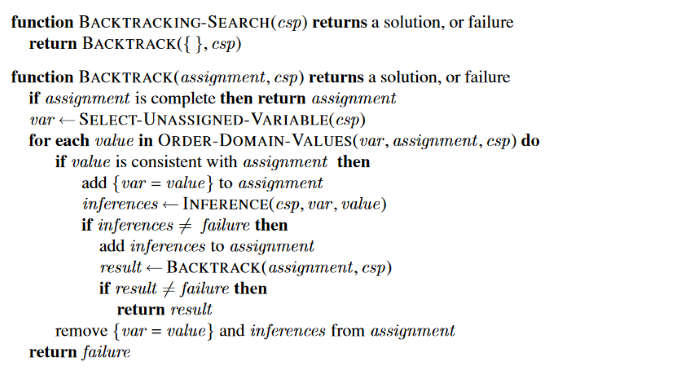
\includegraphics[scale=0.8]{./images/csp.png}
	\captionof{figure}{Pseudocódigo del algoritmo de satisfacción de restricciones implementado.}\label{fig:csp}
\end{center}

\subsubsection{Metaheurísticas:}

\paragraph{El uso de metaheurísticas es uno de los principales aspectos de este trabajo. Su uso está ligado principalmente a los proceso de optimización, que pueden incluir desde una política de negociación de un agente humano, hasta las optimizaciones llevadas a cabo en los experimentos que se realicen con un entorno.}

\paragraph{Una de las metaheurísticas utilizadas fue una variante de algoritmo genético como una forma de modelar la política de negociación de un agente humano, específicamente aquellos que pertenecen a la clase social media, es decir aquellos cuya ganacia es menor que el doble del promedio de los ingresos de los humanos y mayor o igual que la media de dichos ingresos solamente. Específicamente en este proyecto, se utilizó dicha variante de algortimo genético para la solución del problema de la mochila con repetición \cite{mochilarep}, la cual es una forma de ver el mismo problema de elaborar una solicitud de ofertas a comprar por un humano en un destino específico. La idea con este método es que aquellos que lo ejecuten puedan optimizar principalmente en base a la prioridad de las necesidades sin tener mucho en cuenta el dinero que gastan. En la figura \ref{fig:genal} se muestra el pseudocódigo del algoritmo.}

\begin{center}
	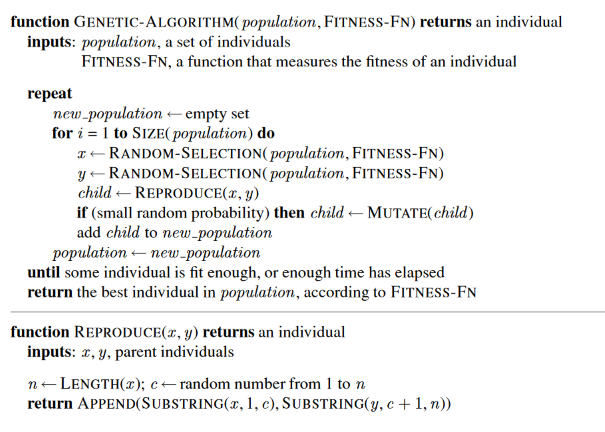
\includegraphics[scale=0.8]{./images/genal.png}
	\captionof{figure}{Pseudocódigo del algoritmo genético.}\label{fig:genal}
\end{center}

\paragraph{Las restantes metaheurísticas están relacionadas con los procesos de optimización, como por ejemplo en la optimización de los experimentos, en cuyo caso se utilizó el algoritmo de \textit{Hill Climbing} \cite{hillclimb} y en la optimización de las compras realizadas por un agente humano, donde se implementó el algoritmo de \textit{Threshold Accepting} \cite{taccept} para aquellos agentes humanos de la clase social más baja, es decir, aquellos cuyos ingresos son menores que la media general de ingresos en la población. La idea de estos algoritmos es poder realizar una optimización eficiente de ciertos parámetros de tal forma que se puedan acotar fácilmente los criterios de parada de los mismos, por lo que el costo computacional puede considerarse asumible.} \label{par:hill}

\subsubsection{Procesamiento de Lenguaje Natural:}

\paragraph{Una de las aplicaciones más importantes del procesamiento de lenguaje natural es la generación de texto, la cual es una tarea que tiene como objetivo la producción controlada de texto que cumpla con cierta estructura y restricciones predefinidas. Para llevar a cabo este enfoque se utiliza un modelo lingüístico formal, el cual puede basado en una gramática que formalice el lenguaje que se intenta generar.}

\paragraph{El problema que se logró solucionar con este método es el de generar nombres de lugares de destino, de forma tal que se disponga con una vía de identificar los agentes de destino con mayor legibilidad al mostrar las notificaciones de las acciones que ocurren durante una simulación. Para ello se construyó una gramática, se creó una pequeña base de nombres de dueños y tipos de destinos, y con el uso de la biblioteca $NLTK$ se logró implementar de manera sencilla dicho algoritmo de generación.}

\subsubsection{Modelos de Markov:}

\paragraph{Los modelos de Markov son una forma bastante común y relativamente simple de modelar estadísticamente procesos aleatorios. Se han utilizado en muchos dominios diferentes, desde la generación de texto hasta el modelado financiero. En general, las Cadenas de Markov son conceptualmente bastante intuitivas y son muy accesibles en el sentido de que pueden implementarse sin el uso de conceptos estadísticos o matemáticos avanzados. Son una excelente manera de comenzar a aprender sobre técnicas de modelado probabilístico y ciencia de datos.}

\paragraph{En el caso específico de este proyecto, se utilizó un modelo de Markov \cite{markovm} ya empleado en otros estudios relacionados con la generación de nombres de personas. Por lo cual, este mismo resultado se utilizó para a generación de identificadores legibles para los agentes humanos que participan en la simulación.}

\subsection{Aplicaciones de la Simulación:}

\paragraph{Existen una serie de elementos pertenecientes al campo de estudio de la Simulación que sería relevante resaltar, lo cual tiene como fin brindar un mayor entendimiento del modelo implementado. Esta constituye una vía de justificar en base a conocimientos bien establecidos, el porqué de varias decisiones durante la realización del proyecto. Por lo tanto, se hace necesaria la mención de algunos de los más importantes.}

\subsubsection{Características del sistema modelado:}

\begin {enumerate}
				\item {\textit{Dinámico no estacionario}: La estructura del sistema cambia con el tiempo y los procesos del sistema ocurren en y dependen de el tiempo.}
				\item {\textit{No determinista}: Conocemos la estructura del sistema y las funciones de cambio de estado y de salida son funciones no deterministas.}
				\item {\textit{Información completa}: Los agentes humanos tienen conocimiento total del estado del sistema. Aunque no ocurre lo mismo con los agentes destino.}
				
\end {enumerate}

\begin {enumerate}
				\item {\textit{Dinámico no estacionario}: La estructura del sistema cambia con el tiempo y los procesos del sistema ocurren en y dependen de el tiempo.}
				\item {\textit{No determinista}: Conocemos la estructura del sistema y las funciones de cambio de estado y de salida son funciones no deterministas.}
				\item {\textit{Información completa}: Los agentes humanos tienen conocimiento total del estado del sistema. Aunque no ocurre lo mismo con los agentes destino.}
				
\end {enumerate}

\subsubsection{Generación de variables aleatorias:}

\paragraph{La generación de variables aleatorias se ve presente en varias secciones del proyecto. Los resultados de la generación de estas pueden encontrarse en varios estudios de referencia \cite{vars1} \cite{vars2} \cite{vars3}. Algunas de las principales son:}

\begin {enumerate}
				\item Tiempo de atención (en minutos) de los lugares de destino a los agentes humanos.
				\item Tiempo de funcionamiento (en horas) de los agentes de destino durante la simulación.
				\item Ingreso monetario de los agentes humanos.
				\item Capacidad monetaria de los agentes humanos.
				\item Distribución de las necesidades de los agentes humanos.
				\item Distribución de las ofertas en los agentes de destino.
				\item Velocidad (en metros por segundo) de traslación de los agentes humanos.
				\item Generación de la longitud de las calles de las ciudades.
\end {enumerate}

\subsubsection{Eventos discretos:}

\paragraph{Los eventos discretos son utilizados específicamente en la forma en que se tratan las colas en los agentes de destino y actualizan los estados de estas a lo largo el tiempo. Como conocemos, en varias de las simulaciones basadas en eventos discretos se tienen tres tipos de variables principales: la variable de tiempo (representada por el campo \textit{next\_available\_time}), las variables contadoras (campo \textit{number\_current\_client}) y las variables de estado del sistema (campos \textit{offers}, \textit{budget} y \textit{queue}). En el caso específico de los agentes de destino, estos contituyen un sistema de atención de un solo servidor, además, los mismos pueden ser vistos a su vez como un modelo de inventario, ya que internamente tiene el seguimiento de un conjunto de productos, los cuales son ofertados a un precio determinado por unidad.}

\subsubsection{Sistema multiagente, comunicación e interacción:}

\paragraph{En este proyecto se cuenta con la implementación de dos tipos de agentes, \textit{HumanAgent} y \textit{DestinationAgent}, de los cuales ya se habló en la sección \ref{subsubsec:agents}. Ahora, resulta importante describir con más detalle las características principales de dichos agentes, la forma de ejecución de sus funcionalidades principales y las interacciones entre estos. Primeramente, cabe destacar que ambos son agentes con estados, ya que los mismos tienen un conocimiento de ciertas variables producto de un conjunto de iteraciones realizadas en el ambiente, por ejemplo, los agentes humanos en cada momento de la simulación conocen el dinero que poseen, las necesidades que les quedan por satisfacer y la posición donde se encuentran en el ambiente,  mientras que por otro lado, los agentes de destino conocen el estado de las ofertas que tienen disponibles y el tiempo transcurrido desde que comenzaron a ejecutarse. Añadido a lo anterior, ambos agentes tienen la capacidad de almacenar un conjunto de acciones realizadas por estos en un momento determinado, por lo cual es posible acceder al historial de acciones de estos.}


	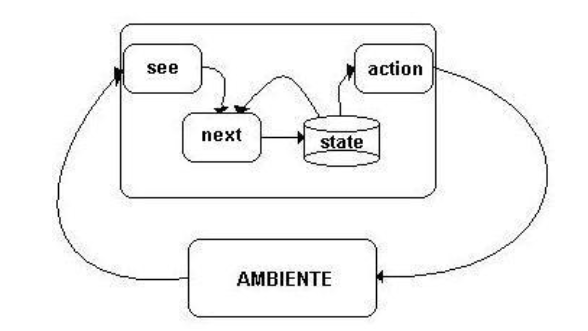
\includegraphics[scale=0.7]{./images/stateagents.png}
	\captionof{figure}{Arquitectura genérica de los agentes con estados.}\label{fig:stateagents}


\paragraph{En el caso de los agentes humanos, estos pueden ser clasificados como proactivos de razonamiento práctico, ya que tienen la funcionalidad de decidir, momento a momento, qué acción realizar para lograr sus objetivos (en este caso, el conjunto de necesidades que poseen).  Estos agentes pueden estar solamente en tres estados para la toma de decisiones: en sus hogares (inicio de la simulación), después de haber realizado una compra en un destino o haber arribado a uno de estos. En el primer caso, la acción la lógica del agente consiste en recibir el estado actual del entorno y determinar el destino al cuál debería ir para satisfacer sus necesidad de acuerdo al criterio que este siga. En el segundo caso, el agente decidirá exactamente lo mismo que en el primero, aunque si ocurre que se haya quedado sin dinero o ya haya visitado todos los  destinos posibles, este terminaría su ejecución. Finalmente, en el tercer caso, el agente recibiría del entorno el estado actual del destino en el que se encuentre, del cual podrá conocer si al momento de su llegada el mismo está lleno o ya su horario de funcionamiento expiró, en cuyo caso tratará de dirigirse a otro destino, mientras que en otro caso, este intentará satisfacer sus necesidades en dicho centro.}

\begin{center}
	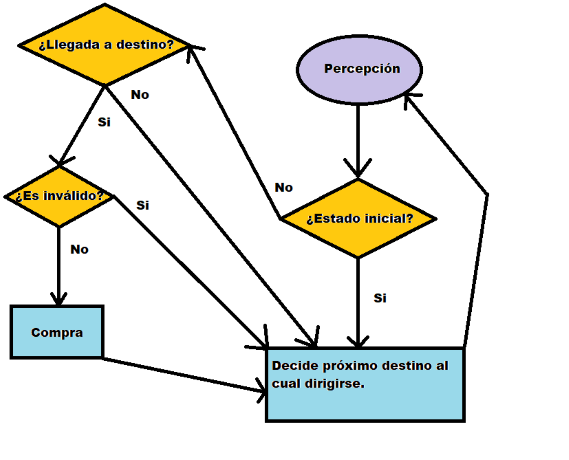
\includegraphics[scale=0.8]{./images/humanalgo.png}
	\captionof{figure}{Algoritmo de comportamiento de los agentes humanos.}\label{fig:humanalgo}
\end{center}

\paragraph{Por otro lado, los agentes de destino reaccionan a peticiones que reciben de compra de artículos o a la llegada de un agente humano al mismo, por lo tanto pueden ser considerados como agentes reactivos. En el primer caso, estos tratarán de validad la compra y actualizar el estado interno del humano, mientras que en el segundo caso estos tratan de encolar al agente humano en su sistema interno de atención.}

\begin{center}
	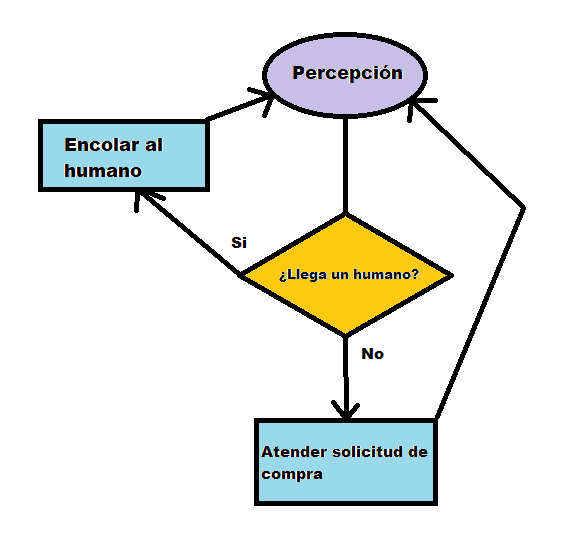
\includegraphics[scale=0.8]{./images/destalgo.png}
	\captionof{figure}{Algoritmo de comportamiento de los agentes de destino.}\label{fig:destalgo}
\end{center}

\subsubsection{Sistema multiagente, comunicación e interacción:}

\paragraph{El sistema que se modela en este proyecto contituye evidentemente un sistema multiagente \cite{multiagent}, ya que el mismo está constituído por un conjunto de agentes (agentes humanos y de destino), cada uno con determinadas capacidades (moverse, negociar, realizar compras, responder a solicitudes de compras) y recursos computacionales (necesidades, dinero, ofertas) para la solución de una clase de problemas o tareas (compra y venta de productos). E objetivo de este sistema es la solución de problemas inherentemente distribuídos, donde los agentes que intervienen en el mismo deben interactuar entre ellos (negociación entre agentes humanos y de destino) de forma tal que esto conduzca a la solución de dichos problemas.}

\paragraph{El principal proceso de interacción entre los agentes humanos y de destino es la negociación. En este, los agentes humanos revisan las ofertas que posee el destino, y realizan una política específica para seleccionar aquellas ofertas que mejor satisfacen su estado actual en base a algún criterio específico. Posteriormente, los agentes de destino reciben dicha solicitud de compra y actualizan, en caso de que esta sea válida, el estado interno de sus ofertas. Finalmente, una vez terminado este proceso, el agente humano trata de determinar el próximo destino al cual dirigirse.}

\subsection{Ejecución de la Simulación:}

\paragraph{La ejecución de la simulación de un entorno es controlada internamente por el campo \textit{schedule} en la clase \textit{Enviroment}. Dicho campo es una cola de prioridad que almacena las acciones que deben ocurrir durante la simulación. Estas acciones son tuplas de la forma \textit{(tiempo, humano, acción, destino)}, donde \textit{tiempo} representa el momento en que debe ejecutarse la acción, \textit{humano} es el agente humano que interviene en la acción, \textit{acción} es el suceso que debe ejecutarse y \textit{destino} es el agente de destino que interactuará con el agente humano.}

\paragraph{Para la simulación se tienen implementadas dos acciones principales, las cuales determinan los cambios de estado en el sistema que se está tratando. Estas son: $arrival$ (encargada de simular el proceso en que un agente humano llega a un agente de destino y se decide si incluirlo en la cola o decidir el próximo destino al cual viajar) y $negotiation$ (simula la situación en que el cliente debe ser atendido por el agente de destino y comienta la fase de negociación).}

\paragraph{En el momento inicial de la simulación cada uno de los agentes humanos está en su hogar, por lo que la primera acción de todos los agentes ería determinar el primer destino al cual dirigirse y luego, el propio sistema se encarga de colocar en la cola de prioridad general dicha acción como un $arrival$, donde el tiempo en que se ejecutaría sería el tiempo en que demora el agente humano en moverse desde su posición actual hasta dicho destino teniendo en cuenta su velocidad y la distancia a recorrer. En un primer momento, todas las acciones serían solamente de movimientos de los agentes humanos hacia centros de destino. La cola de prioridad interna toma el primero de dichos arribos y lo ejecuta. Cada acción de arribo puede generar una acción de compra ($negotiation$) en caso de que el agente decida hacer la cola en dicho centro. En caso contrario se generaría una acción de arribo a otro destino de ser posible. Luego, las acciones de compra son las encargadas de simular toda la lógica de adquisición de productos por parte del humano y una vez terminado este suceso, se procede a generar una acción de arribo de dicho cliente a otro posible destino.}

\begin{center}
	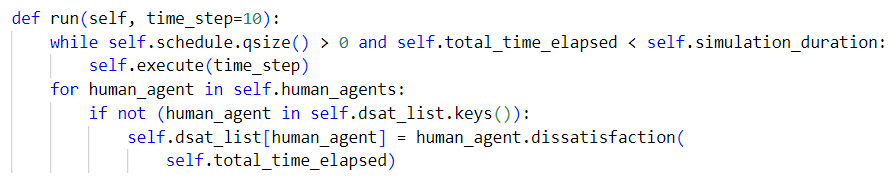
\includegraphics[scale=0.7]{./images/runenv.png}
	\captionof{figure}{Algoritmo de ejecución del entorno.}\label{fig:runenv}
\end{center}

\paragraph{En la figura \ref{fig:runenv} se muestra la implementación en \textit{Python} de la ejecución del entorno. Básicamente, dicho método consiste en ejecutar las acciones en la cola de prioridad de acciones mientras no se cumplan los criterios de parada establecidos.}

\paragraph{Una vez descrita la forma de ejecución de la clase \textit{Environment}, solo quedaría analizar la ejecución de la clase \textit{Experiment}. Esta última es la encargada de obtener una serie de conclusiones interesantes de los entornos realizando siempre un mínimo de $30$ simulaciones. Para inicializar un experimento solo es necesario pasarle a su constructor un entorno ya definido, el cual será la base del mismo. Como se explicó en la sección \ref{par:exp}, esta clase es utilizada para modelar los experimentos basados en diversos criterios de optimización. Para cada uno de los criterios mencionados se ejecuta el algoritmo \textit{Hill Climbing} ya mencionado en \ref{par:hill}. En total dicha clase cuenta con cuatro métodos de optimización, uno por cada factor definido en \ref{par:exp}.}

\begin{center}
	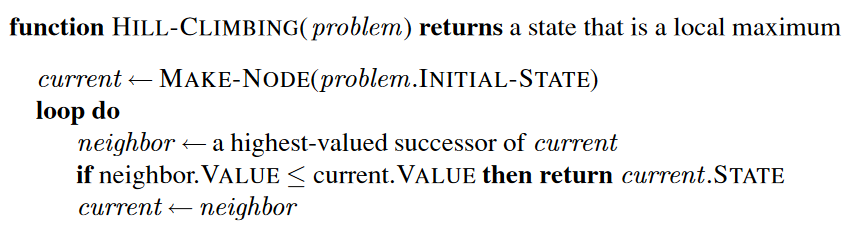
\includegraphics[scale=0.7]{./images/hillclimbp.png}
	\captionof{figure}{Pseudocódigo al algoritmo \textit{Hill Climbing}.}\label{fig:hillclimbp}
\end{center}

\subsection{Resultados de la Simulación:}

\paragraph{Para la ejecución de la simulación primeramente crearemos una instancia de la clase \textit{Environment} con los siguientes parámetros:}

\begin{center}
	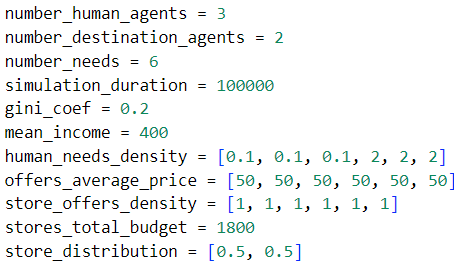
\includegraphics[scale=0.7]{./images/envparams.png}
	\captionof{figure}{Parámetros para la ejecución del entorno.}\label{fig:envparams}
\end{center}

\paragraph{El parámetro \textit{gini\_coef} es sencillamente el coeficiente de Gini \cite{vars2} de la ciudad o región analizada. El coeficiente de Gini es una medida de la desigualdad de una población, indicada como la diferencia entre el área de la curva de la igualdad total y el área de la curva de la distribución real de los ingresos. Debe ser un valor real entre $0$ y $1$, sin incluir el $1$. En el caso de \textit{mean\_income}, esta la media de los ingresos de la región estudiada. Se usa junto al coeficiente de Gini para modelar los ingresos del área analizada.}

\paragraph{El valor \textit{offers\_average\_price} es la media de los precios del producto que suple cierta necesidad en la región estudiada. Para cada necesidad, en su índice específico, se tiene el valor promedio del costo de satisfacer una unidad de esa necesidad. Este dato es almacenado en una lista de valores reales de tamaño igual a la cantidad de necesidades.}

\paragraph{Los parámetros \textit{human\_needs\_density} y \textit{store\_offers\_density} son medidores de la proporción de una necesidad/producto en una persona/tienda. El primero se refiere a la proporción entre la media de la generación de una necesidad en específico en la población estudiada y la media global. Por citar ejemplos, en una población de Cuba se consume mucho más arroz en promedio que a nivel del hemisferio occidental o a nivel mundial o en una población de EE.UU. se consume mucho más papel sanitario en promedio que a nivel mundial. Por otro lado, \textit{store\_offers\_density} es una proporción entre los propios productos de un agente destino, significando que el valor esperado de la proporción entre las existencias de un par de productos es igual a la proporción entre los valores de las densidades asociadas. Ambas variables son listas de valores reales de tamaño igual a la cantidad de necesidades.}

\paragraph{Finalmente,  \textit{stores\_total\_budget} y  \textit{store\_distribution} son los parametros que caracterizan el presupuesto de todos los agentes destino del área estudiada. El primero indica el presupuesto global con el que se compran los productos que se encuentran disponibles a comprar por los agentes humanos, y el segundo indica la distribución de este presupuesto entre todos los agentes destino. El parámetro \textit{stores\_total\_budget}  es un valor real y \textit{store\_distribution} es una lista de valores reales de tamaño igual a la cantidad de agentes destino.}

\paragraph{Primeramente se realizaron $10$ pruebas con el entorno creado, donde en cada una se realizaron unas $30$ simulaciones sobre el mismo. En las figuras \ref{fig:meanresults} y \ref{fig:varresults} se muestra el comportamiento de la media y la varianza de la insatisfacción de los agentes humanos. Como vemos, dichos gráficos prueban la intuición de que con el aumento de las iteraciones, el nivel de descontento de los agentes diminuye, lo cual refleja que estos con el decursar del tiempo logran satisfacer sus necesidades, lo cual prueba la correctitud de la simulación del entorno.}

\begin{center}
	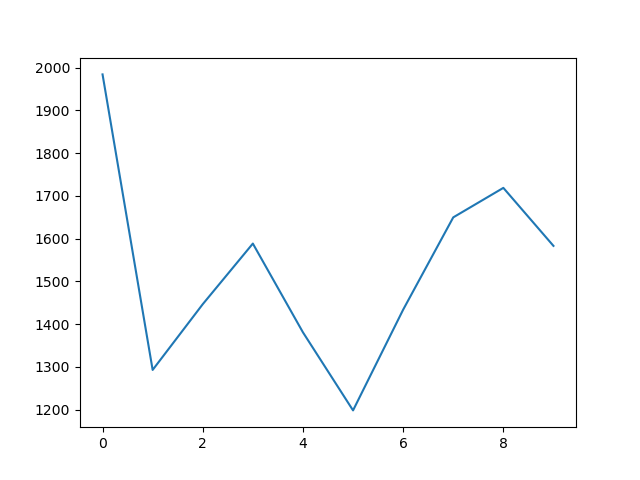
\includegraphics[scale=0.7]{./images/meanresults.png}
	\captionof{figure}{Comportamiento de la media de la insatisfacción de los agentes humanos por cada iteración.}\label{fig:meanresults}
\end{center}

\begin{center}
	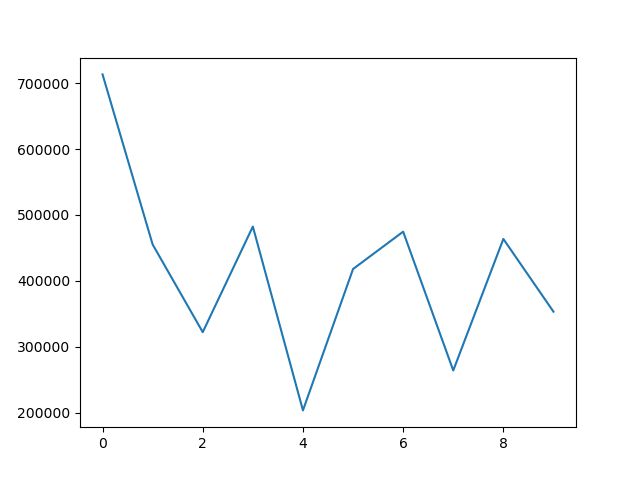
\includegraphics[scale=0.7]{./images/varresults.png}
	\captionof{figure}{Comportamiento de la media de la insatisfacción de los agentes humanos por cada iteración.}\label{fig:varresults}
\end{center}

\subsection{Ejecución de los experimentos:}

\paragraph{Luego de comprobar la ejecución de una instancia de la clase \textit{Enviromnet}, procederemos a inicializar un objeto de tipo \textit{Experiment} co el cual podamos realizar las optimizaciones propuestas en este trabajo:}

\begin {enumerate}
				\item {STORE\_OFFERS\_DENSITY:  En este caso, el valor inicial de \textit{store\_offers\_density} fue $[1, 1, 1, 1, 1, 1]$ con evaluación $1330.30$. La media y la varianza obtenidas para la insatisfacción fueron $1330.30$ y $317205.72$. Al finalizar la optimización, el parámetro estudiado terminó con el valor $[1.33, 1.60, 2.03, 0.17, 0.08, 0.76]$ con una evaluación de $1238.58$ de media de insatisfacción.}
				\item {OFFERS\_PRICE\_FACTOR: El parámetro \textit{store\_offers\_density} comienza con valor $1$ y un factor de penalización de $2.71$. Al finalizar la optimización, \textit{store\_offers\_density} valía $4.73$ mientras que la penalización era de $1.23$. Es importante recordar que este factor hace referencia al valor que se multiplica al precio base de los productos. Como se observa en los resultados, al aumentar el costo de los productos aumenta la insatisfacción, pero la función de penalidad implementada disminuye su valor, de esta forma se explican los resultados obtenidos.}
				\item {TOTAL\_BUDGET\_FACTOR: Es conocido que este factor hace referencia al multiplicador del presupuesto total de los agentes destino. Este comenzó con valor $1$ y un factor de penalización de $2.71$. Al finalizar la optimización, el parámetro tenía un valor de $0.086$ mientras que la penalización era de $1.09$. Como se observa en los resultados, al disminuir la oferta de productos aumenta la insatisfacción, pero la función de penalidad implementada disminuye su valor, de esta forma se explican los resultados obtenidos.}
				\item {STORE\_DISTRIBUTION: En este caso el \textit{Hill Climbing} optimiza sobre el parámetro \textit{store\_distribution}, donde se realizan $40$ iteraciones y en cada una se ejecuta $40$ veces el entorno. La media y la varianza obtenidas para la insatisfacción fueron $1390.97$ y $254075.39$. El estado inicial fue establecido con el valor $[0.5, 0.5]$ para el parámetro \textit{store\_distribution}, con una insatisfacción de $1390.97$, mientras que el estado final estableció que el valor óptimo de \textit{store\_distribution} es $[0.5, 0.5]$, con una insatisfacción de $1262.98$.}
\end {enumerate}

\section{Conclusiones}

\paragraph{Con la realización de este proyecto se logró diseñar un modelo capaz de simular un entorno donde un conjunto de personas se traslada hacia destinos posibles con el fin de satisfacer sus necesidades. Además, gracias a los resultados del análisis estadístico sobre la insatisfacción de los agentes humanos, se pudo probar la calidad de la implementación de los entornos. Finalmente, con la ejecución de los experimentos, se demostró la posibilidad de optimizar factores como la distribución de ofertas en las tiendas y el gasto del presupuesto inicial con una complejidad computacional asumible.}

\section{Recomendaciones}

\paragraph{Se recomienda continuar con el estudio de los procesos relacionados con el movimiento de personas en ciudades con el objetivo de satisfacer necesidades. Resulta de interés ampliar el estudio de este campo a situaciones en las que intervegan la propagación de enfermedades, sistemas de transporte, reabastecimiento de los centros durante el día, simulación de entornos basados en días consecutivos, diseños de sistemas expertos que sirvan de oráculos para la toma de decisiones de los agentes e incluso la aplicación de estos resultados a modelos de escala regional, lo cual traería consigo significativos resultados para empresas, instituciones y gobiernos encargados de diversos centros orientados a la atención de clientes.}

\begin{thebibliography}{99}
	\bibitem{soa1} Michael Jaros, Monika Di Angelo, Peter Ferschin. \emph{Modeling and Simulation of Pedestrian Behaviour As Planning Support for Building Design}.
		Journal of Economic Interaction and Coordination

	\bibitem{soa2} Paul M. Torrens. \emph{Agent models of customer journeys on retail high streets}.
		The Conference on Pedestrian and Evacuation Dynamics 2014 (PED2014).

	\bibitem{soa3} Aloys W.J. Borgers, I.M.E. Smeets, A.D.A.M. Kemperman, and H.J.P. Timmermans. \emph{Simulation of Micro Pedestrian Behaviour in
Shopping Streets}.
		Urban planning Group, Eindhoven University of Technology, The Netherlands

	\bibitem{soa4} Jan Dijkstra, Harry Timmermans, Joran Jessurun. \emph{Modeling planned and unplanned store visits within a framework
for pedestrian movement simulation}.
		The Conference on Pedestrian and Evacuation Dynamics 2014 (PED2014).

\bibitem{soa5}Tilman A. Schenk, Günter Löffler, Jürgen Rauh. \emph{Agent-based simulation of consumer behavior in grocery shopping
on a regional level}.
		Journal of Business Research 60 (2007) 894 – 903

\bibitem{python} Python. 
	URL: \href{https://www.python.org/}
	  {https://www.python.org/}.
		Consultado en \today.

\bibitem{mochilarep}Gladys Bonilla Enríquez, Diana Sánchez Partida, Santiago Omar Caballer Morales. \emph{Algoritmo genético para el problema logístico de
asignación de la mochila (Knapsack Problem)}.
		Universidad Popular Autónoma del Estado de Puebla A.C., Puebla, Puebla, México

\bibitem{hillclimb} Wikipedia. 
	URL: \href{https://es.wikipedia.org/wiki/Algoritmo\_hill\_climbing}
	  {https://es.wikipedia.org/wiki/Algoritmo\_hill\_climbing}.
		Consultado en \today.

\bibitem{taccept}Gunter Dueck, Tobias Scheuer. \emph{Threshold accepting: A general purpose optimization algorithm appearing superior to simulated annealing}.
		Journal of Computational Physics, Volume 90, Issue 1, September 1990, Pages 161-175

\bibitem{markovm} Medium. 
	URL: \href{https://medium.com/@PuchkovOleg/name-generator-tutorial-1c9a3dfb2ab0}
	  {https://medium.com/@PuchkovOleg/name-generator-tutorial-1c9a3dfb2ab0}.
		Consultado en \today.

\bibitem{vars1} Gallup. 
	URL: \href{https://news.gallup.com/poll/166211/worldwide-median-household-income-000.aspx}
	  {https://news.gallup.com/poll/166211/worldwide-median-household-income-000.aspx}.
		Consultado en \today.

\bibitem{vars2}Thitithep Sitthiyot, Kanyarat Holasut. \emph{A simple method for estimating the Lorenz curve}.
		Humanities and Social Sciences Communications volume 8, Article number: 268 (2021)

\bibitem{vars3}Amir Sohrab Sahaleh, Michel Bierlaire, Bilal Farooq, Antonin Danalet, Flurin Silvan Hänseler . \emph{Scenario Analysis of Pedestrian Flow in Public Spaces}.
		School of Architecture, Civil and Environmental Engineering - ENAC, Mayo 2012

\bibitem{multiagent}Luciano García,  Luis Martí, Luis Orosa. \emph{Temas de Simulación}.
		Facultad de Matemática y Computación. Universidad de la Habana. Página 87.

\end{thebibliography}
\smallskip
\smallskip
\end{document}